\section*{State of the Art}

\subsection*{Hybrid controls}

Other approaches exists for making robots walk on two legs.
Historically passive walkers aims at achieving long walking behavior with
a low energy footprint. This is realized through mechanical storage systems
such as springs (DURUS \cite{reherrealizing}), and efficient transmissions.
In general the control approach tries to consider mainly the centroidal dynamics
and uses stability criteria such as the Lyapunov criteria or the Poincar\'e map.
They are less computationally expensive than optimal control methods.
It has been shown in \cite{RazaviBCG15} that a stability criteria can be found using the method of Poincar\'e on the centroidal momentum.
The authors were then able to implement an efficient controller law from this stability criteria.
The work proposed by \cite{KaddarAC15} shows how to generate whole body dynamical motion using the same approach but using the whole body dynamic.

Those controllers are less expensive than optimal control because they required $1$  control per phase.
Typically for walking on flat floor, $2$ phases are taken into account: single support and double support phase.
On the contrary, optimal control methods need to discretize the dynamics and then to compute one control variable for each discretization step.
Classically for walking $8$ control variables needs to be computed for one step.

For standard walking the hybrid control is a good method \cite{westervelt2007feedback}.
In fact, in free space with infinite flat ground walking motions can be considered as cyclic.
Periodic phase and dynamics can be extracted from the Newton-Euler equations and in particular from the centroidal momentum.

One major difficulty is that aperiodic gate are complicated to manage as it would need a large number of controllers to drive the robot.
Walking on uneven ground and maneuvering around an obstacles are typical case where the gait is aperiodic \cite{grizzle20103d}.
In this thesis we will have to handle such cases like going through stepping stones or maneuver around obstacles, etc.

One major advantage of this method is that discontinuous phenomena, like impacts when the lands, are easily modeled using hybrid control.
The impacts can then be manage by the controller after they occur.
In the case of optimal control method it is rather expensive to include such phenomena.
However in the context of the \koroibot project the motion we generated are not dynamical enough to consider huge impacts.
To handle the foot landing we design sufficiently smooth trajectories to not provoke this kind of discontinuities in the robot states.
Typically the foot trajectory ends with zero acceleration and velocity.
Moreover, on HRP-2 specifically, there is a closed loop stabilizer which avoid perturbations and fit at best the smooth trajectories.
Hence in this thesis we will focus on using optimal control methods.

\subsection*{Whole body formulations}

\begin{figure}[ht]
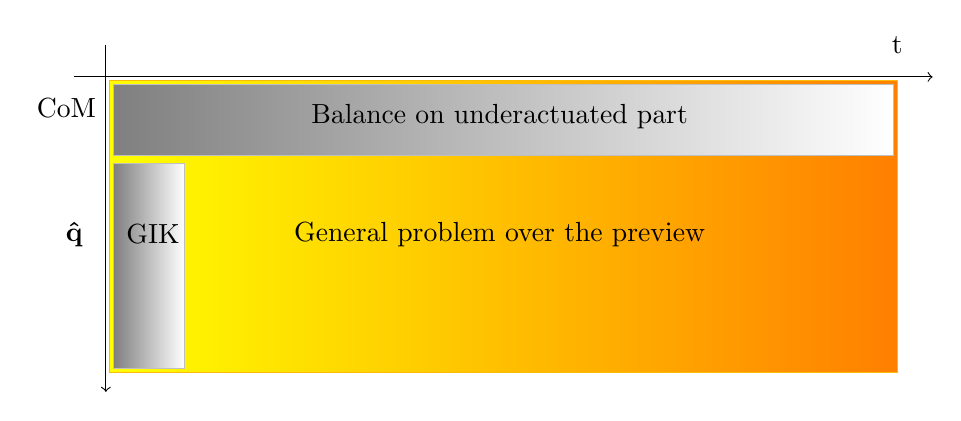
\begin{tikzpicture}
  \draw [->] (-0.4,0) -- (10.5,0);
  \draw [->] (0,0.4) -- (0,-4);
  \shadedraw[left color=yellow, right color= orange, draw=yellow!50!orange](0.05,-0.05) rectangle (10.05,-3.75);
  \shadedraw[left color=gray, right color= white, draw=gray!50!white] (0.1,-0.1) rectangle (10,-1.0);
  \shadedraw[left color=gray, right color= white, draw=gray!50!white](0.1,-1.1) rectangle (1,-3.7);
  \draw (10.05,0.4) node {t};
  \draw (-0.5,-0.4) node {CoM};
  \draw (-0.4,-2.0) node {${\bf \hat{q} }$};
  \draw (5,-0.5) node {Balance on underactuated part};
  \draw (0.6,-2.0) node {GIK};
  \draw (5,-2.0) node {General problem over the preview};
\end{tikzpicture}
\caption{Classical approach (in gray) organization vs. a more global handling of the problem \cite{Todorov:ICRA:2014}}
\label{fig:classical_vs_ddp}
\end{figure}

Fig.~\ref{fig:classical_vs_ddp} depicts the classical approaches used so far.
Indeed the full problem is nonlinear and has around 10 thousand variables and is represented by the whole rectangle.
To be able to solve it researchers used heavy framework for nonlinear optimization.
In fact in \cite{koch:ichr:2014} the authors implemented the above OCP and generated trajectories for the HRP-2 robot.
The software used in this context computes multiple shooting method to solve nonlinear problems.
The solution obtained was a smooth trajectory that allow a HRP-2 robot to step over a $20\,cm$ high obstacle.
The experiment has been done in LAAS-CNRS.
This motion is, for now in LAAS-CNRS, the record in terms of obstacle height.
The bottom heck of this approach is the computation time.
These trajectories took several ours to be computed.
Another formulation implement the complete problem but use simplifications in the contact model.
In \cite{tassa:icra:14} the authors uses Differential Dynamic Programming (DDP) to solve the problem.
This is a very efficient way to compute a solution.
However the current contact model is a spring and damper model.
It produce good enough contact forces to perform multicontact reaching.
However no walking could be performed as the the model provides none dynamically consistent force.
An implementation of this software has been used with HRP-2 in \cite{Koenemann:iros:2015}.
The solver was installed in a remote computer as it still needs multiple powerful CPUs to be used online.
In \cite{Koenemann:iros:2015} the authors used a off board non-real-time Windows
on a $12$-core $4 GHz$ CPU that computes the DDP under $100\,ms$.
The PID controller of the robot runs on an embedded computer using a real time linux with a $2.93\,GHz$ CPU.
The connection between the two computer is done via wifi.

To summarize this, there are not yet powerful techniques that can be used with limited time and computational resources.
As a consequence researchers try to simplify the problem.
The next paragraph presents these approaches.

\subsection*{Mixed formulation}

One simplification consist in taking into account the future of the under-actuated part of the dynamic plus the whole body instantaneous dynamics.
In Fig.~\ref{fig:classical_vs_ddp} this would correspond to the two gray areas but fused together.

During the DARPA robotics challenge the authors of \cite{kuindersma:icra:2014} used a custom active set solver for quadratic programming to solve a mixed formulation.
For the under-actuated formulation they used the seminal work of Kajita \cite{Kajita:icra:2003}.
In addition they used linearized friction cones and optimized the robot joint accelerations.

A recent thesis \cite{phdthesis:sherikov:2016} pursue this work of integrating under-actuated preview control inside a instantaneous whole body controller.
The main difference between Sherikov and Kuindersma's work is the under-actuated model predictive control used.
In fact the walking task of the Sherikov's framework is able to automatically find the foot steps following the formalism of \cite{herdt:iros:2010}.
In Kuindersma's framework the foot steps are precomputed by a planner.

\subsection*{Walking patterns in 3D}

From this subsection on, the hypothesis of separating the under-actuated and whole body motion is made.
The hypothesis is most used in the literature and correspond to the two separated gray rectangles in Fig.~\ref{fig:classical_vs_ddp}.
This means that trajectories for the CoM, the free flyer and the end effectors are computed first.
And only afterward the whole body control is deduced from these preliminary calculations.
The work presented in this section are locomotion algorithm allowing multiple contacts.

An iterative scheme is proposed in \cite{Hirukawa:icra:2007} that can be written as an implicit optimization scheme whose cost function is the distance to a given CoM trajectory and given forces distributions. The resulting forces satisfies \eqref{eq:conic_constraint} by construction of the solution. There is no condition on the angular momentum \eqref{eq:angular:momentum} neither on the viability of the final state \eqref{eq:term_constraint}, however the reference trajectory enforced by the cost function is very likely to play the same role.

In \cite{qiu_dhm11}, \eqref{eq:conic_constraint} is explicitly handled (using the classic linear approximation of the quadratic cones). As in \cite{perrin_isrr15}, \eqref{eq:term_constraint} is indirectly handled by minimizing the jerk. No condition on the angular momentum \eqref{eq:angular:momentum} is considered. Additionally, the proposed cost function maximizes the robustness of the computed forces $\bm\phi$ and minimizes the execution time. Finally, constraints are added to represent the limitation of the robot kinematics.

In \cite{perrin_isrr15}, $\dot \am$ is null by construction of the solution. Moreover, \eqref{eq:conic_constraint} is supposed to always hold by hypothesis and is not checked, while \eqref{eq:term_constraint} is not considered but tends to be enforced by minimizing the norm of the jerk of the CoM, like in \cite{Kajita:icra:2003}. These assumptions result in an (bilinear)-constrained quadratic program that is solved by a dedicated numerical method.

In \cite{rotella_humanoid15}, \eqref{eq:conic_constraint} is handled under a simple closed form solution, while \eqref{eq:term_constraint} is not considered. To stabilize the resolution, the cost function tends to stay close to an initial trajectory of both the CoM and the angular momentum, computed beforehand from a kinematic path. Consequently, \eqref{eq:angular:momentum} is not considered either (as it will simply stay close to the initial guess).

\subsection*{Walking patterns in 2D}
In addition to the previous remarks, another difficulty is the bilinear form of the dynamics \eqref{eq:angulardyn}.
When the contacts are all taken on a same plane, a clever reformulation of the dynamics makes it linear \cite{Kajita:icra:2003}, by neglecting the dynamics of both the CoM altitude and the angular momentum. In that case, \eqref{eq:angulardyn} boils down to the constraint of the center of pressure point (CoP) to be in the support polygon.

Kajita et al. \cite{Kajita:icra:2003} did not explicitly check the constraint \eqref{eq:conic_constraint}.
In exchange, $\ell_u$ is used to keep the control trajectory close to a reference trajectory provided a priori.
Similarly, \eqref{eq:term_constraint} is not checked either.
In exchange, $\ell_x$ tends to stabilize the robot at the end of the trajectory by minimizing the jerk of the CoM.
These three simplifications turns \eqref{eq:ocpgen} into a simple unconstrained problem of linear-quadratic regulation that is implicitly solved by integrating the corresponding Riccati equation.
Interesting motions can be perform using this walking pattern generator.
\cite{evrard2009intercontinental} shows that tele-cooperation was possible using humanoid robot and teh walking pattern generator from \cite{Kajita:icra:2003}.

The LQR was reformulated into an explicit OCP \cite{herdt:ar:2010}, directly solved as quadratic program.
The OCP formulation makes possible the formulation of inequality constraints.
\eqref{eq:conic_constraint} is then explicitly checked under its CoP form.

A modification of this OCP is proposed in \cite{Sherikov:ichr:2014} where \eqref{eq:term_constraint} is nicely approximated by the capturability constraint, which is a linear constraint on the CoM and its first time derivative in case of 2D contacts.

\subsection*{Computing the contact placements}

When considering an explicit OCP formulation, additional static variables can be added to the problem.
Typically, the placement of the contact, that are given as invariant in \eqref{eq:ocpgen}, might be computed at the same time.
This was first proposed in \cite{herdt:ar:2010} for a 2D WPG, and similarly used in \cite{Sherikov:ichr:2014} and other works by the same authors.
Similarly, it was proposed in \cite{rotella_humanoid15} to include it in the proposed 3D WPG, but this feature was not implemented nor demonstrated.
In both cases, the placements of the contacts are unlimited (or similarly limited to a convex compact set).
The problem becomes much harder when the contacts might be taken among a discrete set of placements.
In \cite{deits:ichr:14}, the problem was formulated has a mixed-integer program (i.e. having both continuous and discrete variables) in case of flat contact, and solved using an interior-point solver to handle the discrete constraints.
In \cite{mordatch:tog:12}, the same problem is handled using a dedicated solver relying on a continuation heuristic, and demonstrated for animating the motion of virtual avatars.

This is not an exhaustive bibliography.
Many papers need to be cited but also replaced in their scientific context.
So for sake of clarity, a more detailed bibliography is written at the beginning of each chapter.
This allow a better understanding on the state-of-art which is specific to each chapter of this thesis.
